 % !Mode:: "TeX:UTF-8"
\RequirePackage[l2tabu, orthodox]{nag}
\documentclass[a4paper, 10pt]{article}

%%%% PACKAGES %%%%
\usepackage[T1]{fontenc}
\usepackage{amsmath, amssymb, amsthm}
\usepackage[table,usenames,dvipsnames]{xcolor}
\usepackage[utf8]{inputenc}
\usepackage[english]{babel}
\usepackage{placeins}
\usepackage{graphicx}
\usepackage{url}
\usepackage[colorlinks=true]{hyperref}
\usepackage{fancyhdr}
\usepackage{lastpage}
\usepackage{paralist}
\usepackage{parskip}
\usepackage[justification=justified,singlelinecheck=false]{caption}
\usepackage{algorithm}
\usepackage{algpseudocode}
\usepackage{fullpage}
\usepackage{lmodern}
\usepackage[nounderscore]{syntax}
\usepackage{lipsum}
\usepackage{multicol}
\usepackage{float}
\usepackage[framemethod=TikZ]{mdframed}
\usepackage{booktabs}
\usepackage{cleveref}
\usepackage[colorinlistoftodos]{todonotes}

%%%% PACKAGE SETTINGS & GENERAL ALTERATIONS %%%%

% Page margins
\renewcommand{\headrulewidth}{0in}
\setlength\headsep{40pt}
\setlength\headheight{20pt}
\addtolength{\textheight}{-20pt}
\setlength{\columnsep}{20pt}

% Boxed floats
%\floatstyle{boxed}
%\restylefloat{figure}

% MD Frames
\mdfdefinestyle{stubFrame}{%
    linecolor=red,
    linewidth=3pt,
    leftmargin=1cm,
    innerleftmargin=20pt,
    innerrightmargin=20pt,
    rightmargin=1cm,
    topline=false,
    bottomline=false}
\mdfsetup{skipabove=\topskip,skipbelow=\topskip}

\mdfdefinestyle{theoremstyle}{%
    linecolor=red,linewidth=2pt,%
    frametitlerule=true,%
    frametitlebackgroundcolor=gray!20,
    innertopmargin=\topskip,
}


%%%% FILL THESE OUT %%%%
\newcommand{\mySubject}{Advanced Algorithms: Notes}
\newcommand{\myLocation}{DIKU}
\newcommand{\myAuthor}{Martin Grünbaum (martin@itsolveonline.net)}
\newcommand{\myShortAuthor}{Martin G.}

% \maketitle-related
\title{Advanced Algorithms: Notes}
\author{Author: \myAuthor}

% Fancy header
\pagestyle{fancy}
\lhead{\footnotesize \myShortAuthor\\\ }
\chead{\footnotesize\mySubject}
\rhead{\footnotesize\myLocation\\\today}
\cfoot{Page \thepage}

% Document-specific commands


\begin{document}
    \maketitle
    \thispagestyle{empty}
    \pagebreak
    \pagestyle{empty}
    \tableofcontents
    \pagebreak
    \setcounter{page}{1}
    \pagestyle{fancy}
    \section{Max-flow}
%%
A flow network $G = (V,E)$ is a directed graph where each edge $(u,v) \in E$ has
a non-negative capacity $c(u,v) \geq 0$. If there is an edge $(u,v) \in E$ then
there is no edge $(v,u) \in E$. If $(u,v) \notin E$ then $c(u,v) = 0$ for convenience.
When $(u,v) \notin E$, $f(u,v) = 0$.

Flow networks have a source $s$ and a sink $t$. For each vertex $v \in V$, the flow
network contains a path $s \leadsto v \leadsto t$. The graph is therefore connected, meaning
$|E| \geq |V| - 1$.

A flow is a real-valued function $f : V \times V \rightarrow \mathbb{R}$ that satisfies
two properties:
%%
\begin{description}
	\item[Capacity constraint:] For all $u,v \in V$, $0 \leq f(u,v) \leq c(u,v)$

	\item[Flow conservation:] For all $u \in V - \{s,t\}$, 
	$\sum_{v \in V} f(u,v) = \sum_{v \in V} f(v,u)$.
\end{description}
%%
The value of a flow, $|f|$, is defined as:
%%
\begin{align*}
	|f| = \sum_{v \in V} f(s,v) - \sum_{v \in V} f(v,s)
\end{align*}
%%
In the \textbf{maximum-flow} problem, we are given a flow network $G$ and we wish to find
a maximum flow.

Edges are anti-parallel if there is both an edge $(u,v)$ and an edge $(v,u)$. This is not allowed,
and to get around this we instead introduce a new edge $x$ and re-structure the edges as follows:
$(u,x), (x,v), (v,u)$. The capacity of the new edges involving $x$ is the same as the capacity from
$(u,v)$. See page 711 in the book for an example.

\subsection{Multiple sources and sinks}
%%
This can be accounted for by introducing a \textbf{supersink} and \textbf{supersource} with infinite
flow and capacity out to all of the sources and from all of the sinks to the supersink. See page 713.

\subsection{Ford-Fulkerson}
%%
Three basic principles: \textbf{residual networks}, \textbf{augmenting paths} and \textbf{cuts}.
Essential for \textbf{max-flow min-cut} theorem (Theorem 26.6).

Intuition is as follows: We have a flow network $G$. We iteratively alter the flow of $G$, 
by finding an augmenting path in an associated residual network $G_f$. Once we know the edges
that belong to an augmenting path, we can identify specific edges in $G$ to increase or decrease
the flow of. Each iteration increases overall flow, but it may do so by decreasing the flow along
certain edges. This is repeated until the residual network $G_f$ has no more augmenting paths.

\textbf{max-flow min-cut} shows that upon termination, this yields a maximum flow.

\subsubsection{Residual network}
\begin{figure}
	\centering
	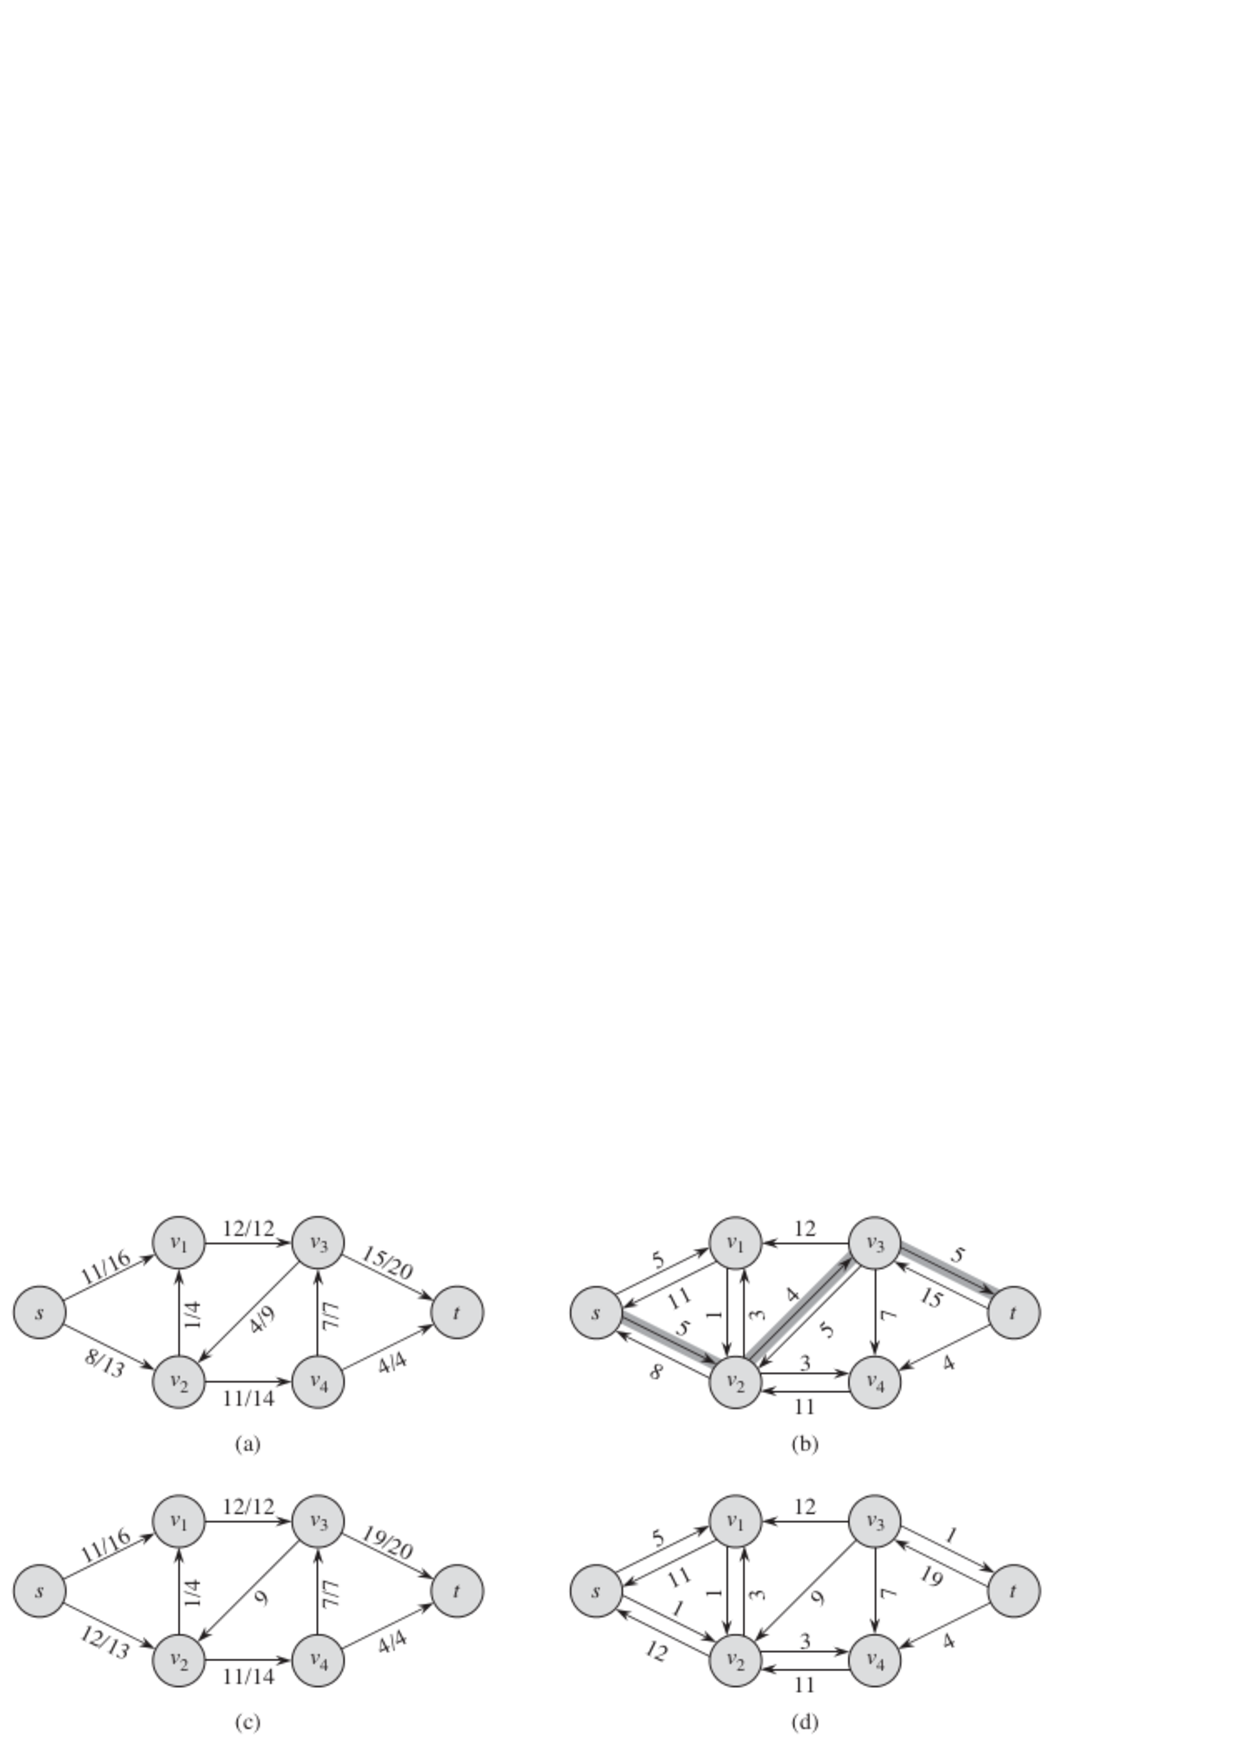
\includegraphics[width=\textwidth]{images/augmenting_paths}
\end{figure}
%%
Given a network $G = (V,E)$ with a flow $f$, the \textbf{residual network}
of $G$ induced by $f$ is $G_f = (V, E_f)$, where
%%
\[
	E_f = \{(u,v) \in V \times V : c_f(u,v) > 0\}.
\]
%%
Residual capacity $c_f(u,v)$ is defined by
%%
\[
 c_f(u,v) =
  \begin{cases}
  	c(u,v) - f(u,v) & \text{if } (u,v) \in E, \\
  	f(v,u) & \text{if } (v,u) \in E, \\
  	0 & \text{otherwise}
  \end{cases}
\]
%%
\textit{Note:} that $(u,v) \in E$ implies $(v,u) \notin E$, so there is always only one of the three
above cases that applies. 

Because the edges in $E_f$ are either edges from $E$ or an edge in the opposite direction,
$|E_f| \leq 2|E|$.

Intuition: A residual network $G_f$ consists of edges with capacities that
represent how we can alter the flow on edges of $G$. $G$ can admit an
additional amount of flow along an edge, equal to the capacity minus the
current flow. If the edge can admit more flow, that edge is placed into $G_f$
with a value of $c_f(u,v) = c(u,v) - f(u,v)$. The residual network may also
contain edges that are not in $G$: In order to represent a possible decrease
of a flow $f(u,v)$ on an edge in $G$, we place an edge $(v,u)$ into $G_f$ with
residual capacity $c_f(v,u) = f(u,v)$. In other words, an edge that can admit
flow in the opposite direction, at most cancelling out flow entirely. See
Figure~\ref{fig:aug_paths} for an example.

Flows in a residual network satisfy the definition of a flow, but with respect to capacities
$c_f$ in the network $G_f$. If $f$ is a flow in $G$ and $f'$ is a flow in the corresponding residual
network $G_f$, we define $f \uparrow f'$, the \textbf{augmentation flow} of f by f', as a function
from $V \times V$ to $\mathbb{R}$ defined by
%%
\[
  (f \uparrow f')(u,v) =
  \begin{cases}
  	f(u,v) + f'(u,v) - f'(v,u) & \text{if } (u,v) \in E, \\
  	0 & \text{otherwise.}
  \end{cases}
\]

Intuition: Increase the flow ($f(u,v)$) by $f'(u,v)$, but decrease it by the flow in the
opposite direction ($f'(v,u)$). Pushing flow in the reverse direction is also called \textbf{cancellation}.

\subsubsection{Augmenting path}
An augmenting path $p$ is a simple path from $s$ to $t$ in the residual network $G_f$. By the definition
of a residual network, we may increase the flow of an edge $(u,v)$ by up to $c_f(u,v)$ without violating the
capacity constraint on whichever of $(u,v)$ and $(v,u)$ is in the original flow network $G$.

The maximum amount by which we can increase flow on each edge of an augmenting path $p$ is the
\textbf{residual capacity} of $p$, given by $c_f(p) = min\{c_f(u,v) : (u,v) \text{ is on p}\}$. More specifically,
if $p$ is an augmenting path in $G_f$, we define a function $f_p : V \times V \rightarrow \mathbb{R}$ as
%%%
\[
	f_p(u,v) =
	\begin{cases}
		c_f(p) & \text{if } (u,v) \text{is on } p, \\
		0 & \text{otherwise}.
	\end{cases}
\]
%%
Then $f_p$ is a flow in $G_f$ with value $|f_p| = c_f(p) > 0$. See Lemma 26.2, page 720. It remains to be
shown that augmenting $f$ by $f_p$ produces a different flow in $G$ whose value is closer to the maximum.
Corollary 26.3 on page 720 shows this by immediate proof, using Lemma 26.1 and 26.2.
    \section{Fibonacci heaps: Disposition}
\begin{enumerate}
	\item Mergeable heaps
	\item Structure
	\item Operations
	\begin{itemize}
		\item Make-Heap
		\item Insert
		\item ExtractMin
		\item Union / Merge
		\item DecreaseKey
		\item Delete
	\end{itemize}
\end{enumerate}

CLRS 19

\section{Fibonacci heaps: Notes}

\subsection{Mergeable heaps}
A mergeable heap is one which supports the following operations:
%
\begin{description}
	\item[Make-Heap()] Creates and returns a new heap containing no elements.
	\item[Insert(H,x)] Inserts element $x$, whose key has already been filled in,
	into heap $H$.
	\item[Minimum(H)] Returns a pointer to the element in heap $H$ whose key is minimum.
	\item[Extract-Min(H)] Deletes the element from heap $H$ whose key is minimum,
	returning a pointer to the element.
	\item[Union($H_1$,$H_2$)] Creates and returns a new heap
	that contains all the elements of heaps $H_1$ and $H_2$.
	The original heaps are destroyed by this operation.
\end{description}
%
In addition to the above operations, Fibonacci heaps also
support the following two operations:
%
\begin{description}
	\item[Decrease-Key(H,x,k)] Assigns to element $x$ within
	heap $H$ the new key value $k$, which we assume to be no
	greater than its current key value.
	\item[Delete(H,x)] Deletes element $x$ from heap $H$.
\end{description}

\begin{table}[h!]
\caption{Running time of operations}
\begin{tabular}{ccc}
	Procedure & Binary heap(worst case) & Fibonacci heap (amortized) \\ \hline
	Make-heap & $\Theta(1)$ & $\Theta(1)$ \\
	Insert    & $\Theta(lg\ n)$ & $\Theta(1)$ \\
	Minimum   & $\Theta(1)$ & $\Theta(1)$ \\
	Extract-Min & $\Theta(lg\ n)$ & $\mathbb{O}(lg\ n)$ \\
	Union	& $\Theta(n)$ & $\Theta(1)$ \\
	Decrease-Key & $\Theta(lg\ n)$ & $\Theta(1)$ \\
	Delete & $\Theta(lg\ n)$ & $\mathbb{O}(lg\ n)$
\end{tabular}
\end{table}

Fibonacci heaps are theoretically desirable when the number
of Extract-Min and Delete operations is small relative to the
number of other operations performed. This can be the case for
some algorithms in graph problems, that call decrease-key once
per edge. Fast algorithms for computing minimum spanning trees and
finding single-source shortest paths make essential use of
Fibonacci heaps.

From a practical point of view, however, the constant factors
and complexity of Fibonacci heaps make them less desirable than
ordinary binary (or k-ary) heaps for most applications.
As such, Fibonacci heaps are pre-dominantly of theoretical
interest.

\subsection{Structure of Fibonacci heaps}
A Fibonacci heap is a collection of rooted trees that are
min-heap ordered. Each tree obeys the min-heap property: the
key of a node is greater than or equal to the key of its
parent. Each node contains a pointer to its parent and a pointer
to any one of its children. The children are linked together in
a circular, doubly linked list. In a circular, doubly linked list
we can insert a node into any location or remove a node from
anywhere in the list in $O(1)$ time. We can also concatenate two
such lists in $O(1)$ time. 

Each node also contains the number of children (\textbf{x.degree}) and
a boolean-valued attribute x.mark, to indicate whether it has
lost a child since the last time $x$ was made the child of another
node. Newly created nodes are unmarked, and a node becomes unmarked
whenever it is made the child of another node. Root nodes are unmarked.

We access a Fibonacci heap $H$ by a pointer $H.min$ to the
root of a tree containing the minimum key; we call this node the
minimum node of the Fibonacci heap.

The roots of all the trees in a Fibonacci heap are linked
together using their left and right pointers into a circular,
doubly linked list called the root list of the Fibonacci heap.
Finally, $H.n$ refers to the number of nodes currently in the heap.

In the following, the potential function of $\Phi(H) = t(H) + 2m(H)$ is used,
where $t(H)$ is the number of trees and $m(H)$ is the number of marked nodes.
The potential function captures the state of a system at a given point, and
we can then calculate an amortized time as the actual time plus a constant times
the \textbf{change} in state `energy'. This provides a valid upper bound on running
time.

\subsection{Analysis: Running time of methods}
\subsubsection{Make-Heap}
Creates a fibonacci heap with no trees. This gives a potential energy of
$\Phi(H) = 0$, since $t(H)=0$ and $m(H)=0$. The total running time is thus the
actual cost of $O(1)$.

\subsubsection{Insert}
Insert simply inserts a node as a root-tree in the Fibonacci heap, increasing
the number of trees by one. To determine the amortized cost, let $H$ be the
input Fibonacci Heap and $H'$ be the resulting Fibonacci heap. Then,
$t(H')=t(H)+1$ and $m(H')=m(H)$. The increase in potential is thus: $((t(H)+1)
+ 2m(H)) - (t(H) + 2m(H)) = 1$.

Since the actual cost is $O(1)$, the amortized cost is $O(1) + 1 = O(1)$.

\subsubsection{Find-Min}
We store a pointer to the minimum node of a Fibonacci heap. As the potential
is not changed (we alter no state in the tree), the amortized running time is
the actual cost of $O(1)$.

\subsubsection{Uniting two Fibonacci heaps}
To unite two Fibonacci heaps, we concatenate the root lists of the two heaps
$H_1$ and $H_2$ and then determine the new minimum node. The change in
potential is:
\begin{align*}
	& \Phi(H) - (\Phi(H_1) + \Phi(H_2)) \\
	&= (t(H)+2m(H)) - ((t(H_1)+2m(H_1)) + (t(H_2)+2m(H_2))) \\
	&= 0
\end{align*}
Since $t(H) = t(H_1) + t(H_2)$ and $m(H) = m(H_1)+m(H_2)$. The amortized time
is thus equal to the actual running time of $O(1)$.

\subsection{ExtractMin}
ExtractMin works by first making a root of each of the minimum nodes children
and removing the minimum node from the root list. Then the root list is
consolidated by linking roots of equal degree, until at most one root remains
of each degree. To do this efficiently, an array is created that stores
a current pointer to a root tree of a given degree.

We then consolidate the root list, to reduce the number of trees in the
Fibonacci heap. The following steps are repeatedly executed until every root
in the root list has a distinct degree:
%
\begin{enumerate}
	\item Find two roots $x$ and $y$ in the root list with the same degree. Without loss of generality, let $x.key \leq y.key$.
	\item \textbf{Link} $y$ to $x$: remove $y$ from the root list,
	and make $y$ a child of $x$. Then we increment the attribute
	$x.degree$ and clear the mark on $y$.
\end{enumerate}

The array of degrees -> root pointers is used to look up whether there
is another tree of the same degree as we have just increased $x$ to,
and if there is they link. If not, the entry in the array is updated
to point to $x$.

The root list is then emptied and re-created based on the
pointers in the array of degrees -> root pointers. Finally,
we decrement $H.n$ by 1 and return a pointer to the deleted node.

There are several things we must estimate the cost of:
extracting the minimum node, the main for-loop through the root
list and within that the while-loop that links together trees.

The amortized cost of extracting the minimum node of an $n$-node
Fibonacci heap is $O(D(n))$. Let $H$ denote the
Fibonacci heap prior to the ExtractMin operation. The actual
cost of extracting the minimum node contributes $O(D(n))$ work
from processing at most $D(n)$ chilren of the minimum node.

Upon calling consolidate, the size of the root list is at most $D(n) + t(H) -
1$: the original $t(H)$ root-list nodes, minus the extracted root node, plus
the children of the extracted node, at most $D(n)$. Every iteration of the
inner while-loop, we know that one root is linked to another, and so the total
number of iterations of the while loop over all iterations of the for loop is
at most the number of roots in the root list. Hence, the total amount of work
performed in the for loop is at most proportional to $D(n) + t(H)$. The total
actual work in extracting the minimum node is therefore $O(D(n) + t(H))$. The
potential before extracting the minimum node is $t(H) + 2m(H)$. The potential
afterwards is at most $(D(n)+1)+2m(H)$, since at most $D(n)+1$ roots remain and
no nodes get marked during this operation. The amortized cost is thus at most:

\begin{align*}
	& O(D(n)+t(H)) + ((D(n)+1) + 2m(H)) - (t(H)+2m(H)) \\
	=& O(D(n)) + O(t(H)) - O(t(H)) \\
	=& O(D(n))
\end{align*}
if we scale up the units of the potential to dominate the constant hidden in $t(H)$.
We will see later that $D(n) = O(lg\ n)$, giving an amortized running time of $O(lg\ n)$
for extracting the minimum node.

\subsubsection{DecreaseKey}
DecreaseKey on a node $x$ (with parent $y$) works as follows: Decrease the key
of $x$. If $x$.key < $y$.key, cut $x$ and turn it into a root-node. Then perform
a cascading cut on $y$ upwards, which will cut any node that is already marked,
terminating when it reaches a root node or an unmarked node. Reaching an unmarked node
will mark it. Finally, we check whether $x.key$ < $H.min.key$, and if so update $x$ to
be the minimum node of $H$.

This process means that a node can lose one child (causing it to be marked), but losing
another will cause it to be cut as it was already marked from losing a child before.

DecreaseKey takes $O(1)$ time, plus the time to perform the cascading cuts. Each recursive
call of cascading cut also takes $O(1)$ time, giving $O(c)$ for $c$ cascading cuts. The actual
time of DecreaseKey, including recursive calls, is thus $O(c)$.

The call to cut $x$ creates a new tree rooted at $x$ and clears $x$'s mark bit (which may have
been false already). Each call of cascading cut, except for the last one, cuts a marked node and
clears its marked bit. Afterwards, the Fibonacci heap contains $t(H)+c$ trees (the original $t(H)$ trees,
$c-1$ trees produced by cascading cuts and the tree rooted at $x$). It contains at most 
$m(H)- c + 2$ marked nodes ($c-1$ nodes were unmarked by cascading cuts and the last call may have marked
a node). The change in potential is therefore, at most:
\[
	((t(H)+c) + 2(m(H) - c + 2)) - (t(H) + 2m(H)) = 4 - c
\]

This leads to an amortized cost of at most:
\[
	O(c) + 4 - c = O(1)
\]
since, again, we can scale up the units of the potential to dominate the constant hidden in $O(c)$.

\subsubsection{Delete}
Deleting a node works by first setting its key to minus infinity, and then extracting the minimum.
We already know that decreasing a key takes $O(1)$ amortized time, and extracting minimum takes
$O(D(n))$ amortized time. As we will see that $D(n) = O(lg\ n)$, deleting a node runs in amortized
time of $O(lg\ n)$

\subsection{Bounding the maximum degree of a Fibonacci heap}
\todo[inline]{Pages 523 - 526 of Lemma's and corollaries, need to be written and explained!}
    \section{NP-Completeness: Disposition}
\begin{enumerate}
	\item The intuition behind NP-Complete problems
	\item 
\end{enumerate}
    \section{Randomized Algorithms: Disposition}
\begin{enumerate}
	\item Randomized Quicksort
	\item Las Vegas, Monte Carlo
	\item 1-sided vs. 2-sided
	\item Bounding running times
	\item Markov \& Chebyshev's inequalities
	\item Randomized Selection
\end{enumerate}

Motwani \& Raghavan Ch. 1.1, 1.2, Ch. 3.2, 3.3

\section{Randomized Algorithms: Notes}

\subsection{Randomized quicksort}
In randomized quicksort, we wish to sort a set of numbers $S$ into ascending
order. We first select a pivot $y$ from $S$ at random. Subsequently, each
remaining element is compared to $y$ and put into $S_1$ if smaller, $S_2$
otherwise. We recursively sort $S_1$ and $S_2$ in the same manner, and then
output $S_1$ followed by $y$ followed by $S_2$.

The running time of randomized quicksort is analyzed in terms of the number of
comparisons made, as this dominates the running time of any (reasonably designed)
algorithm. In particular, we wish to find the \textit{expected} number of comparisons
made.

For $1 \leq i \leq n$, let $S_{(i)}$ denote the element of rank $i$ (the $i$th smallest element)
in the set $S$. Thus, $S_{(1)}$ denotes the smallest element and $S_{(n)}$ the largest. Define the
random variable $X_{ij}$ to assume the value $1$ if $S_{(i)}$ and $S_{(j)}$ are compared in an execution
and the value $0$ otherwise.

The total number of comparisons is then $\sum_{i=1}^n \sum_{j>i} X_{ij}$. The expected number of comparisons is
then $\mathbb{E}[\sum_{i=1}^n \sum_{j>i} X_{ij}] = \sum_{i=1}^n \sum_{j>i} \mathbb{E}[X_{ij}]$ by Linearity
of Expectation.

Let $p_{ij}$ denote the probability that $S_{(i)}$ and $S_{(j)}$ are compared in an execution. $X_{ij}$ can
assume the values $0$ and $1$, so:

\[
	\mathbb{E}[X_{ij}] = p_{ij} \times 1 + (1 - p_{ij}) \times 0 = p_{ij}
\]

To facilitate determining $p_{ij}$, we view the execution of randomized quicksort as a binary search tree $T$, where
each node is a distinct element of $S$. The root of the tree is the pivot $y$ we choose initially; the left sub-tree
contains elements in $S_1$ and the right sub-tree elements in $S_2$. The structure of the sub-trees is determined
recursively by subsequent runs of randomized quicksort. Importantly, the root of the tree ($y$) is compared to elements
in $S_1$ and $S_2$, but elements in $S_1$ are never compared to elements in $S_2$. Thus, there is a comparison between
an $S_{(i)}$ and $S_{(j)}$ only if one is the ancestor of the other.

This makes $T$ a random binary search tree. We are for this analysis interested in the level-order traversal of the
nodes of $T$. Such a traversal is a permutation $\pi$ obtained by visiting the nodes of $T$ in increasing order of
the level numbers, and in a left-to-right order within each level; recall that the $i$th level of the tree is the set
of all nodes at distance exactly $i$ from the root node.

To compute $p_{ij}$ we make use of two observations:
%
\begin{enumerate}
	\item There is a comparison between $S_{(i)}$ and $S_{(j)}$ if and only if $S_{(i)}$ or $S_{(j)}$ occur
	earlier in the permutation $\pi$ than any element $S_{(l)}$ such that $i < l < j$. Intuitively, they are
	only compared if there is some pivot node $l$ that puts $i$ in $S_1$ and $j$ in $S_2$. To see this, let
	$S_{(k)}$ be the earliest in $\pi$ from among all elements of rank between $i$ and $j$. If $k \notin \{i,j\}$
	then $S_{(i)}$ will belong to the left sub-tree of $S_{(k)}$ while $S_{(j)}$ will belong to the right sub-tree
	of $S_{(k)}$, implying that there is no comparison between $S_{(i)}$ and $S_{(j)}$. Conversely, if
	$k \in \{i,j\}$ then it must be that there is a parent-child relationship between $S_{(i)}$ and $S_{(j)}$
	implying that the two are compared.

	\item Any of the elements $S_{(i)}, S_{(i+1)}, \hdots, S_{(j)}$ is equally likely to be chosen as the pivot and
	hence appear first in $\pi$. Thus, the probability that the first element is either $S_{(i)}$ or $S_{(j)}$ is
	exactly $2 / (j - i + 1)$.
\end{enumerate}
%
This establishes that $p_{ij} = 2/(j - i + 1)$. The expected number of comparisons is thus:
%
\begin{align*}
	\sum_{i=1}^n \sum_{j>i} p_{ij} &= \sum_{i=1}^n \sum_{j>i} \frac{2}{j-i+1} \\
	&\leq \sum_{i=1}^n \sum_{k=1}^{n-i+1} \frac{2}{k} \\
	&\leq 2\sum_{i=1}^n \sum_{k=1}^{n} \frac{1}{k}
\end{align*}
%
It follows that the expected number of comparisons is bounded by $2nH_n$, where $H_n$ is the \textit{nth}
Harmonic number, defined by $H_n = \sum_{k=1}^n 1/k$. We know that $H_n \sim ln\ n + \Theta(1)$, making the
expected running time of randomized quicksort $O(n\ lg\ n)$

\subsection{Las Vegas \& Monte-Carlo}
An algorithm that \textit{always} gives the correct solution, but whose running time is variable or perhaps even
unbounded, is a \textbf{Las Vegas} algorithm. In contrast, an algorithm that may sometimes produce an incorrect
solution (although we can often bound the probability of this), but we know will always terminate, is a
\textbf{Monte-Carlo} algorithm. One useful property of a Monte-Carlo algorithm is that we can reduce the risk of
failure to be arbitrarily small by running the experiment repeatedly with
independent random choices each time.

For decision problems (yes or no problems), there are two kinds of Monte-Carlo
algorithms: those with one-sided error and those with two-sided error. A
Monte-Carlo algorithm is said to have a two-sided error if there is a non-zero
probability that it errs when it outputs either \texttt{YES} or \texttt{NO}. It is said
to have one-sided error if the probability that it errs is zero for at least one of the
possible outputs (\texttt{YES} / \texttt{NO}).

By definition, a Las Vegas algorithm is a Monte-Carlo algorithm with error
probability $0$. We say that a Las Vegas algorithm is an \textit{efficient}
Las Vegas algorithm if on any input its expected running time is bounded by a
polynomial function of the input size. Similarly, we say that a Monte-Carlo
algorithm is an \textit{efficient} Monte-Carlo algorithm if on any input its
worst-case running time is bounded by a polynomial function of the input size.

\subsubsection{Markov \& Chebyshev's inequalities}
\begin{description}
\item[Markov inequality] Let $Y$ be a random variable assuming only non-negative
  values. Then for all $t \in \mathbb{R}^+$,
  \[
    \text{Pr}[Y \geq t] \leq \frac{\text{E[Y]}}{t}.
  \]
  Equivalently,
  \[
    \text{Pr}[Y \geq k\text{E}[Y]] \leq \frac{1}{k}.
  \]
\item[Proof] Define a function $f(y)$:
  \[
   f(y) = \begin{cases}
     1 & \text{iff } y \geq t\\
     0 & \text{otherwise.}
   \end{cases}
  \]
  Then $\text{Pr}[Y \geq t] = \text{E}[f(y)]$. Since $f(y) \leq y/t$ for all $y$,
  \[
    \text{E}[f(Y)] \leq \text{E}\left [\frac{Y}{t} \right ] = \frac{\text{E}[Y]}{t},
  \]
  and the theorem follows. \qed
\end{description}

\begin{description}
\item[Chebyshevs inequality] Let $X$ be a random variable with expectation
  $\mu_X$ and a standard deviation of $\sigma_X$. Then for any $t \in
  \mathbb{R}^+$,
  \[
    \text{Pr}[|X - \mu_X| \geq t\sigma_X] \leq \frac{1}{t^2}
  \]
\item[Proof] Note that
  \[
    \text{Pr}[|X - \mu_X| \geq t\sigma_X] = \text{Pr}[(X - \mu_X)^2 \geq
    t^2\sigma_X^2]
  \]
  The random variable $Y = (X - \mu_X)^2$ has expectation $\sigma_X^2$, and
  applying the Markov inequality to $Y$ bounds this probability from above by
  $1/t^2$. \qed
\end{description}
    %\bibliographystyle{plain}
    %\bibliography{bibliography}
\end{document}